% !TEX encoding = UTF-8
% !TEX TS-program = pdflatex
% !TEX root = ../Articolo.tex
% !TEX spellcheck = it-IT

%************************************************
\section{Behavior Investigation}
\label{section:behaviorinvestigation}
%************************************************

This is the third draft of what should be the main topic of my PhD Thesis. The \textbf{ToC} is developed accordingly and attached, at its end you can also find the \textbf{Bibliography} collected until now.

\subsection{Investigation topcis}
\label{subsection:investigationtopics}

The scientific core of my PhD Thesis will investigate the following themes:
\begin{enumerate}
%\item{the micro-macro transition,}
\item{the influence of variations (distributions) of input parameters and poly-dispersity,}
%\item{the behavior of the different properties in real life (e.g. segregation before doing the shear cell experiment),}
\item{the possbility to extrapolate (e.g. given 3 different fraction distributions, with known behaviors, extrapolate the behavior of a fourth fraction distribution).}
\end{enumerate}


\subsection{Micro - DEM parameters}
\label{subsection:microparameters}

The main micro parameters in a simulation are:

\begin{enumerate}[label=(\Alph*)]
\item{the particle diameter distribution ($radii$ (R),\%) (0.00025 - 0.05 $[m[$),}
\item{the particle density ($\rho_p$) (2000-4000 $[kg/m^3]$),}
\item{the Young modulus ($E$) (10 $[MPa]$),}
\item{the Poisson ratio ($\nu$) (0.4 $[-]$),}
\item{the coefficient of restitution ($e$) (0.1-1.0 $[-]$),}
\item{the sliding friction ($sf$) (0.1-1.0 $[-]$),}
\item{the rolling friction ($rf$) (0.1-1.0 $[-]$),}
\item{the domain edge dimension ($D_{cyl}$), proportional to R (76, 100, 124 times bigger).}
\end{enumerate}

The parameter that drives the simulation time is $D_{cyl}$. The number of particles is cubically proportional to its size. \\
The simulations will be run with defined interval values.\\

\subsection{Macro - bulk parameters}
\label{subsection:macroparameters}

The main macro parameters we experimentally determine for a bulk material are:

\begin{enumerate}[label=(\alph*)]
\item{the particle diameter distribution ($radii$) (0.00001 - 0.05 $[m[$),(\%),}
\item{the bulk density ($\rho_b$) (1000-3000 $[kg/m^3]$),}
\item{the coefficient of restitution ($e$) (0.1-1.0 $[-]$),}
\item{the internal friction angle in different loading and consolidation conditions ($\phi$) (25-50 $[^\circ]$).}
\end{enumerate}


\subsection{Defined intervals simulations}
\label{subsection:definedintervalssimulations}
For the Angle of Repose simulation the individual contacts micro-DEM parameters will be:
\begin{itemize}
\item{Sliding friction: from 0.05 to 1, 0.05 interval $=$ 20 possibilities;}
\item{Rolling friction: from 0.05 to 1, 0.05 interval $=$ 20 possibilities;}
\item{Coefficient  of restitution: from 0.5 to 1, 0.1 interval $=$ 6 possibilities;}
\item{Particle density: e.g. from 2500 to 3500 $kg/m3$, 100 interval $=$ 11 possibilities;}
\item{(Particle to geometry ratio (p2g): 50, 100, 150 $=$ 3 possibilities;)}
\end{itemize}
$20 \cdot 20 \cdot 6 \cdot 11 \cdot 3 = 26400$ possible combinations of parameters.
Each combination would require a simulation, each simulation requires 9 hours over 32 cores $=$ 9900 days!
All for only one material with a defined size distribution (e.g. from 3 to 10 mm)!
We only consider p2g $=$ 50, because otherwise with e.g. 100 the number of particles is 8 times higher, and so the time 8 times longer.

For the Shear cell simulation the individual contacts micro-DEM parameters will be the same of the AOR simulation, plus:
\begin{itemize}
\item{Normal stress: 1, 2, 5, 10 kPa $=$ 4 possibilities;}
\item{Shear \%: 40, 60, 80, 100\% $=$ 4 possibilities;}
\end{itemize}
$20 \cdot 20 \cdot 6 \cdot 11 \cdot 4 \cdot 4 = 422400$ possible combinations of parameters.
Each combination would require a simulation, each simulation requires 64 minutes over 32 cores $=$ 18774 days!
Again all for only one material with a defined size distribution (e.g. from 3 to 10 mm)!


\subsection{Artificial neural network}
\label{subsection:artificialneuralnetwork}

Do we really need all these simulations?
How to identify the effect (weight) each parameter?\\
The representation of a multi-sphere experiment through a mathematical model presents numerous complexities.
A different approach involves an artificial neural network, that can be realized to understand the relationship between the input and the output parameters.
An artificial neural network is composed of many artificial neurons that are linked together according to a specific network architecture. The objective of the neural network is to transform the inputs into meaningful outputs.
The inputs are:
\begin{enumerate}
\item{\textit{A}, from real data \textit{a} but simplified,}
\item{\textit{B,H},}
\item{\textit{C,D}, from literature,}
\item{\textit{E}, from real data \textit{e},}
\item{\textit{F,G}, the main calibration parameters,}
\end{enumerate}
The outputs are \textit{b}, \textit{f} and \textit{g}.\\
The idea would be to use a \textit{feed forward Multi Layer Perceptron Neural Network (MLPNN)}.
A backpropagation reinforcement learning training algorithm has been used (scaled conjugate gradient).\\
A Neural Network (NN) has been created for each bulk parameter investigated ($\mu_{e,ps}$, $\mu_{e,s}$, $\rho_{b}$).
This bulk parameters, or $target$, have been obtained by running a limited number of simulations (for each bulk), $\approx 600$ for the shear cell and 81 for the angle of repose.
Together with the corresponding inputs they have been used to train the networks.\\
15\% of the simulations have been excluded from the training processes.
They have been used to define per each NN the correct number of neurons in the hidden layer, based on an $R^2$ maximization.
Now that the networks have been trained, we can feed the networks with all the combination we need and receive reliable macro-BULK parameters as response.
Especially, we can increase the parameter that account for the geometry dimension, without paying completely the price for it.\\
The NN inputs will be defined interval values or random values.\\

\subsubsection{Defined interval values}
\label{subsubsection:definedintervalvalues}

For the $defined interval values$ procedure each trained NN received as input the $422400$ different combinations.
Then we selected between them the valid $input-DEM-micro$ parameters combinations by fitting NN outputs to experimental data (within a 5\% error).
About $400$ of them were selected.
Next step will be to validate the DEM parameters by means of static angle-of-repose experiments and AOR simulations-trained NN (the $26400$ combinations).\\

Let's say that between the 400 simulations remained, as hypothesis 20 of them are experimentally validated. At this point I should be able to \textit{extrapolate the behavior of bulk with a volume too large to be simulated} with this complete neural network and to compare the results with the real scale experiments (Leoben).\\

The reliability of this work is deeply based on the already performed simulations: further numerical investigations as suggested in draft $1$ could improve it.\\


\subsubsection{Random values}
\label{subsubsection:randomvalues}

For the $random values$ procedure each trained NN received as input the same as the $defined interval values$, except for the following:
\begin{itemize}
\item{Sliding friction: from 0.05 to 1, 100 random numbers, and so 100 possibilities;}
\item{Rolling friction: from 0.05 to 1, 100 random numbers, and so 100 possibilities;}
\item{Coefficient  of restitution: from 0.5 to 1, 50 random numbers, and so 50 possibilities;}
\item{Particle density: e.g. from 2500 to 3500 $kg/m3$, 50 random numbers, and so 50 possibilities.}
\end{itemize}
Together it makes 25 millions different combinations.
Again we selected between them the valid $input-DEM-micro$ parameters combinations by fitting NN outputs to experimental data (within a 5\% error).
About $400$ thousand of them were selected.\\
From them we extracted of the $valid$ input parameters the following values:
\begin{enumerate}
\item{the minimum and the maximum,}
\item{the mean ($\mu$) and the standard deviation ($\sigma$),}
\item{the lines between $p_i$'s,}
\end{enumerate}
as can be seen in Fig. \ref{011testRadar3}

\begin{figure}[!h]
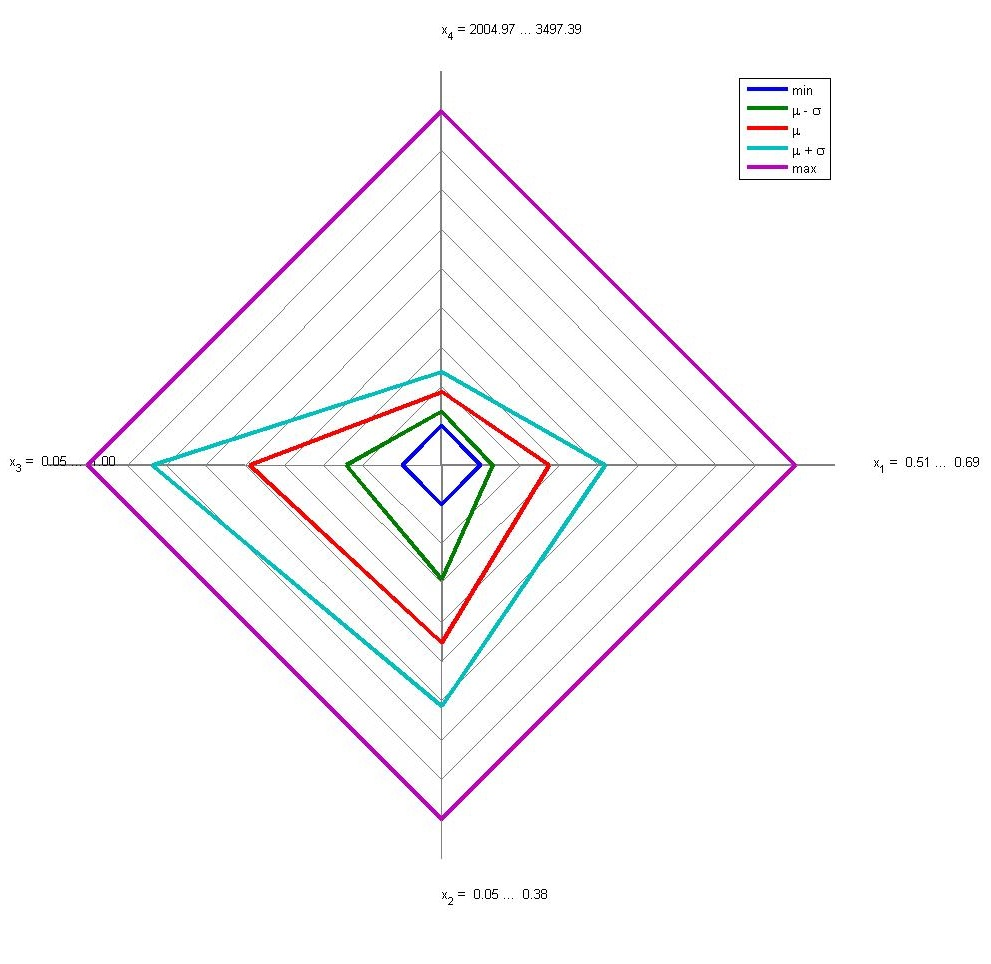
\includegraphics[width=.96\columnwidth]{011testRadar3}
\caption[radar plot of random inputs]{radar plot of random inputs: $X_1 = e$, $X_2 = sf$, $X_3 = rf$, $X_4 = \rho_p$}
\label{011testRadar3}
\end{figure}